\section{Approach Overview}
\label{overview:sec}

{\tool} has two main processes: training and predicting.

\subsection{Training Process}

Figure~\ref{overview-training} displays the general architecture of
{\tool}'s training process. The input of the training process is the
source code of a buggy method and one of its buggy statements, and the
respective fixed source code. If a method has multiple buggy
statements, we treat one buggy statement and that enclosing method at
a time as a training instance. The output includes the trained
tree-based code context learning model (CCL model to learn the
surrounding code context) and the trained tree-based code
transformation learning model (CTL model to learn the
bug-fixing code transformations) with their parameters. The training
process has two main steps:

\begin{figure}[t]
	\centering
	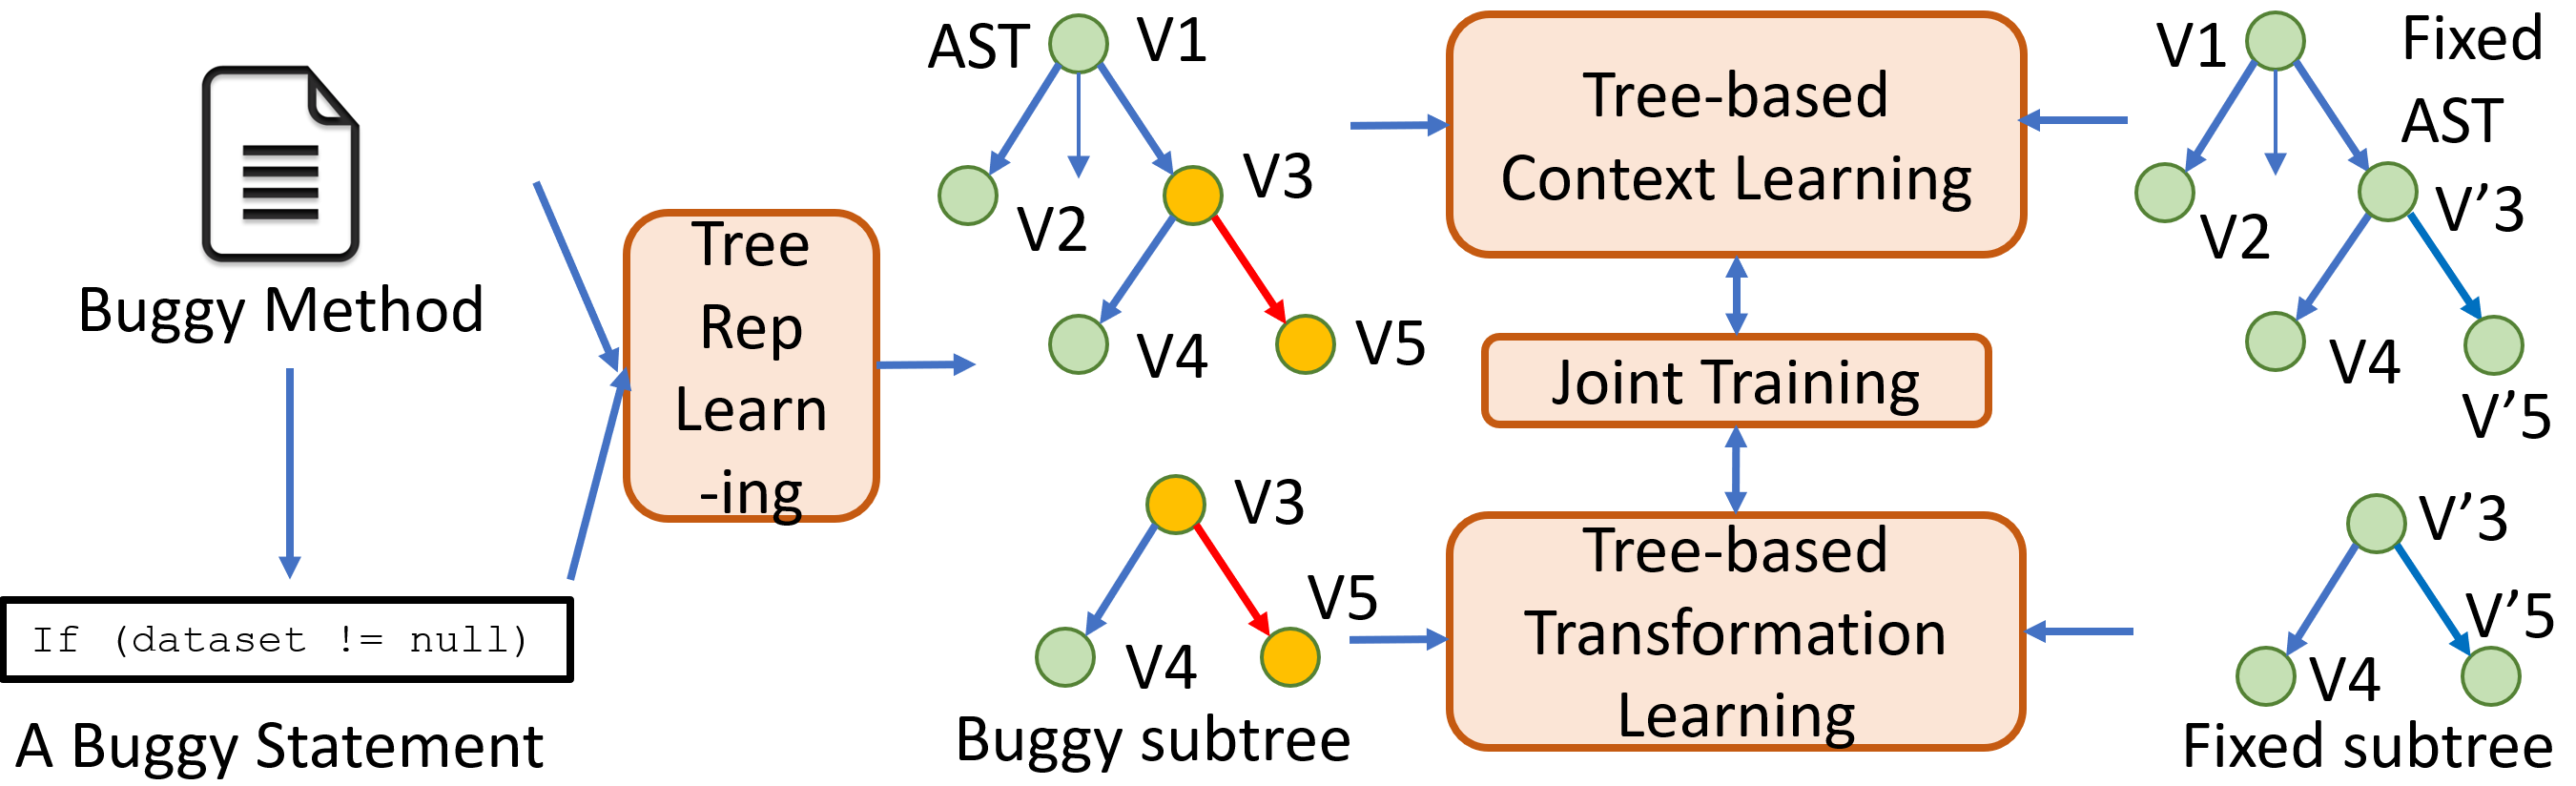
\includegraphics[width=3.4in]{graphs/overview-training.png}
        \vspace{-15pt}
	\caption{{\tool}: Training Process}
	\label{overview-training}
\end{figure}

\vspace{3pt}
\noindent {\bf Tree-based Representation Learning.} The goal of this
step is to take the source code under study and to build the
tree-based vector representations (embeddings) to be the input for our
dual models: CCL and CTL. To achieve that, we first
parse the given source code to obtain the abstract syntax tree (AST)
for the given method and the subtree for the buggy statement.  We
then use a word embedding technique to produce the vector for each
node in the AST when we flatten the AST. The output of this step is
the AST for the method and the AST subtree for the buggy statement in
which each node is replaced by its embedding vector
(Figure~\ref{overview-training}).

\vspace{3pt}
\noindent {\bf Context-aware Dual Learning Automated Program Repair.}
The goal of this step is to train both of the tree-based context
learning model (CCL) and the tree-based code transformation model
(CTL) at the joint training manner. The entire AST $T^{M}_b$ of the
buggy method after vectorization (i.e., each node is a vector) is used
at the input layer of the context learning model (CCL) for
training. The AST of the corresponding fixed method $T^{M}_f$ after
vectorization is used at the output layer of the CCL model. Similarly,
the AST subtree $T^{S}_b$ of the buggy statement after vectorization
is used at the input layer of the transformation learning model (CTL),
and the subtree $T^{S}_f$ of the fixed statement after vectorization
is used at the output layer of the CTL model. Each of the CCL and CTL
models is realized via an attention-based \code{seq2seq} model (we
will explain later). Instead of cascading the two models CCL and CTL,
we use a mechanism called {\em cross-stitch
  unit}~\cite{misra2016cross}, to train them simultaneously with
soft-sharing the parameters to exploit this duality. Joint training is
aimed to learn the shared representations between CCL amd CTL in terms
of a linear combination of the input features in both models. The
output of this step includes the trained CCL and CTL models.

\subsection{Prediction Process}



Figure~\ref{overview-fixing} illustrates the prediction process, i.e.,
the automated fixing process. The input of this process is the buggy
statement in the enclosing method. A common usage of our tool is that
before using {\tool}, a developer could use a fault localization tool
(FL) to detect a buggy statement that needs to be fixed. Another usage
is that a developer can pinpoint the buggy statement and invoke {\tool}
for an auto-fixing suggestion. The fixing process shares the first
step of Tree-based Representation Learning with the training process. After
that step, the vectorized buggy AST subtree (each tree node is
represented by an embedding), is used as the input of the {\em trained
  tree-based transformation learning model} (CTL). The output of the
trained CTL model is the fixed AST subtree, which is converted back
into source code to form a candidate patch. Then, the candidate patch
is validated. We design a novel patch validation scheme that makes use
of beam search for an efficient process. The final candidate patches
are then produced.

\begin{figure}[t]
	\centering
	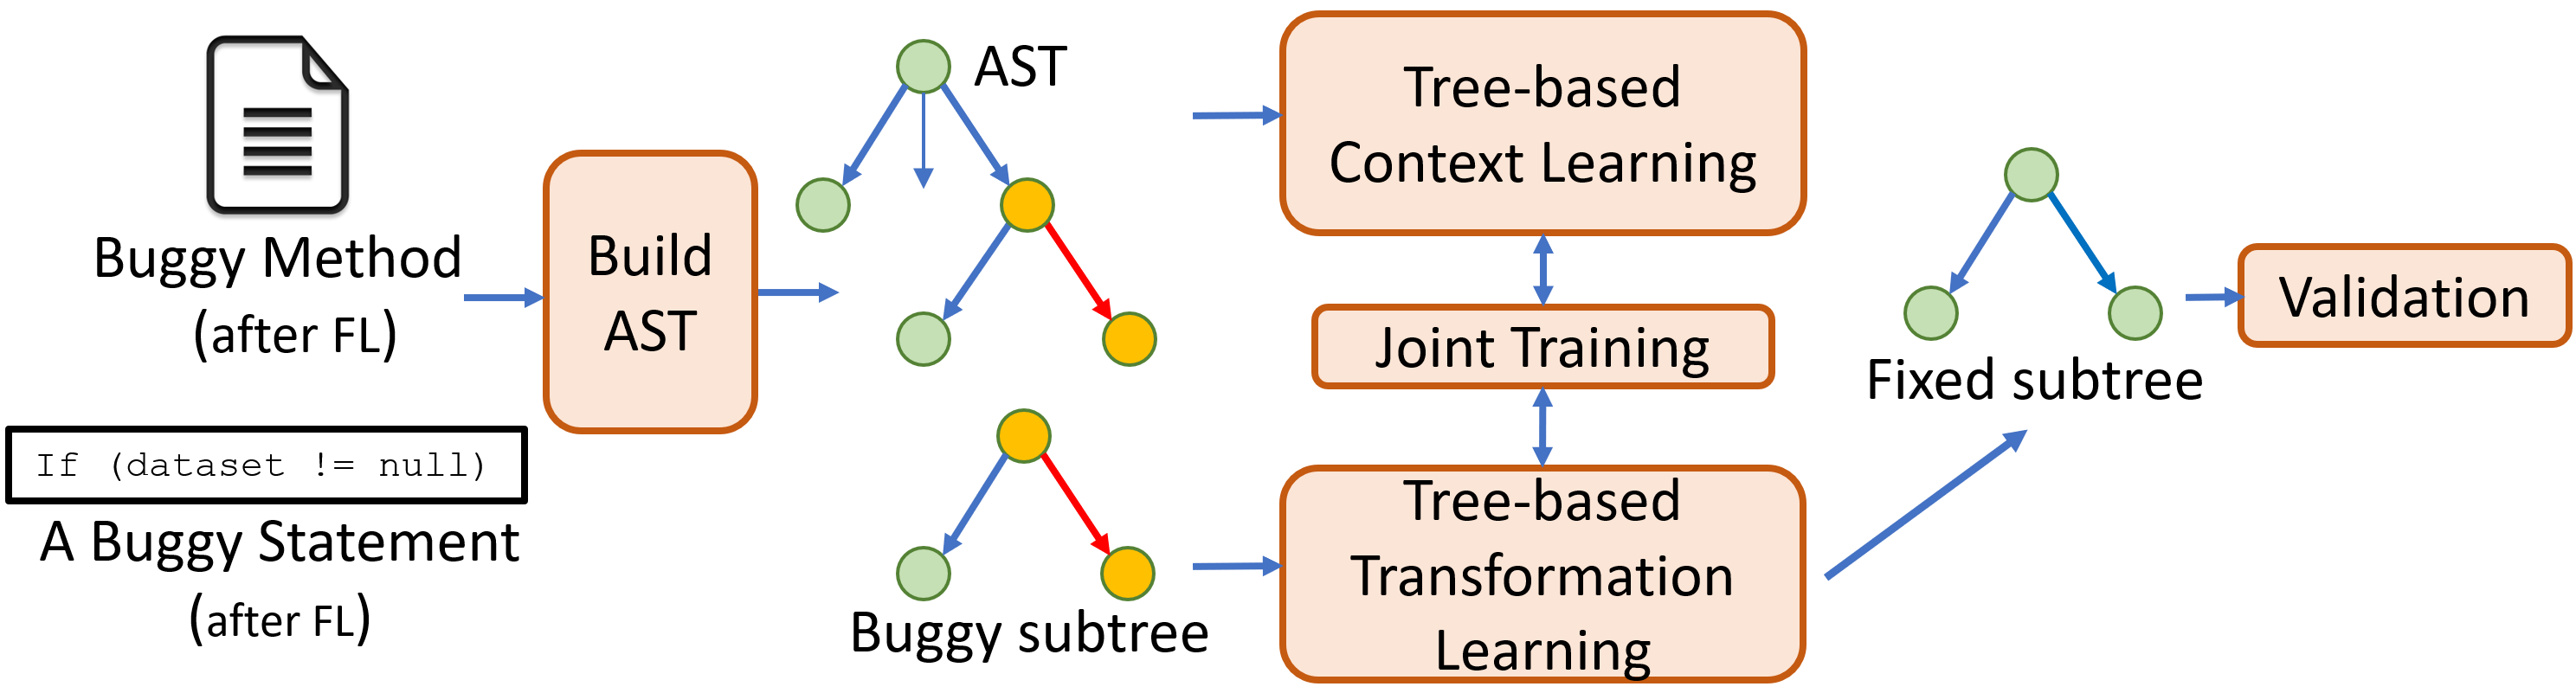
\includegraphics[width=3.4in]{graphs/overview-predict.png}
	\caption{{\tool}: Fixing Process}
        \vspace{-3pt}
	\label{overview-fixing}
\end{figure}
